% src/slides/source/final/core/03_objective.tex

\begin{frame}{Project Objective}
  \SlideBody{\begin{VisualCanvas}
    \node[final statement,text width=14.4cm,
      font=\sffamily\fontsize{16}{20}\selectfont] at (7.4,5.15)
      {Evaluate DiscoNet's Detection Quality and Scalability\\
      under Perfect Communication};
    \node[inner sep=0pt] at (2.4,3.32)
      {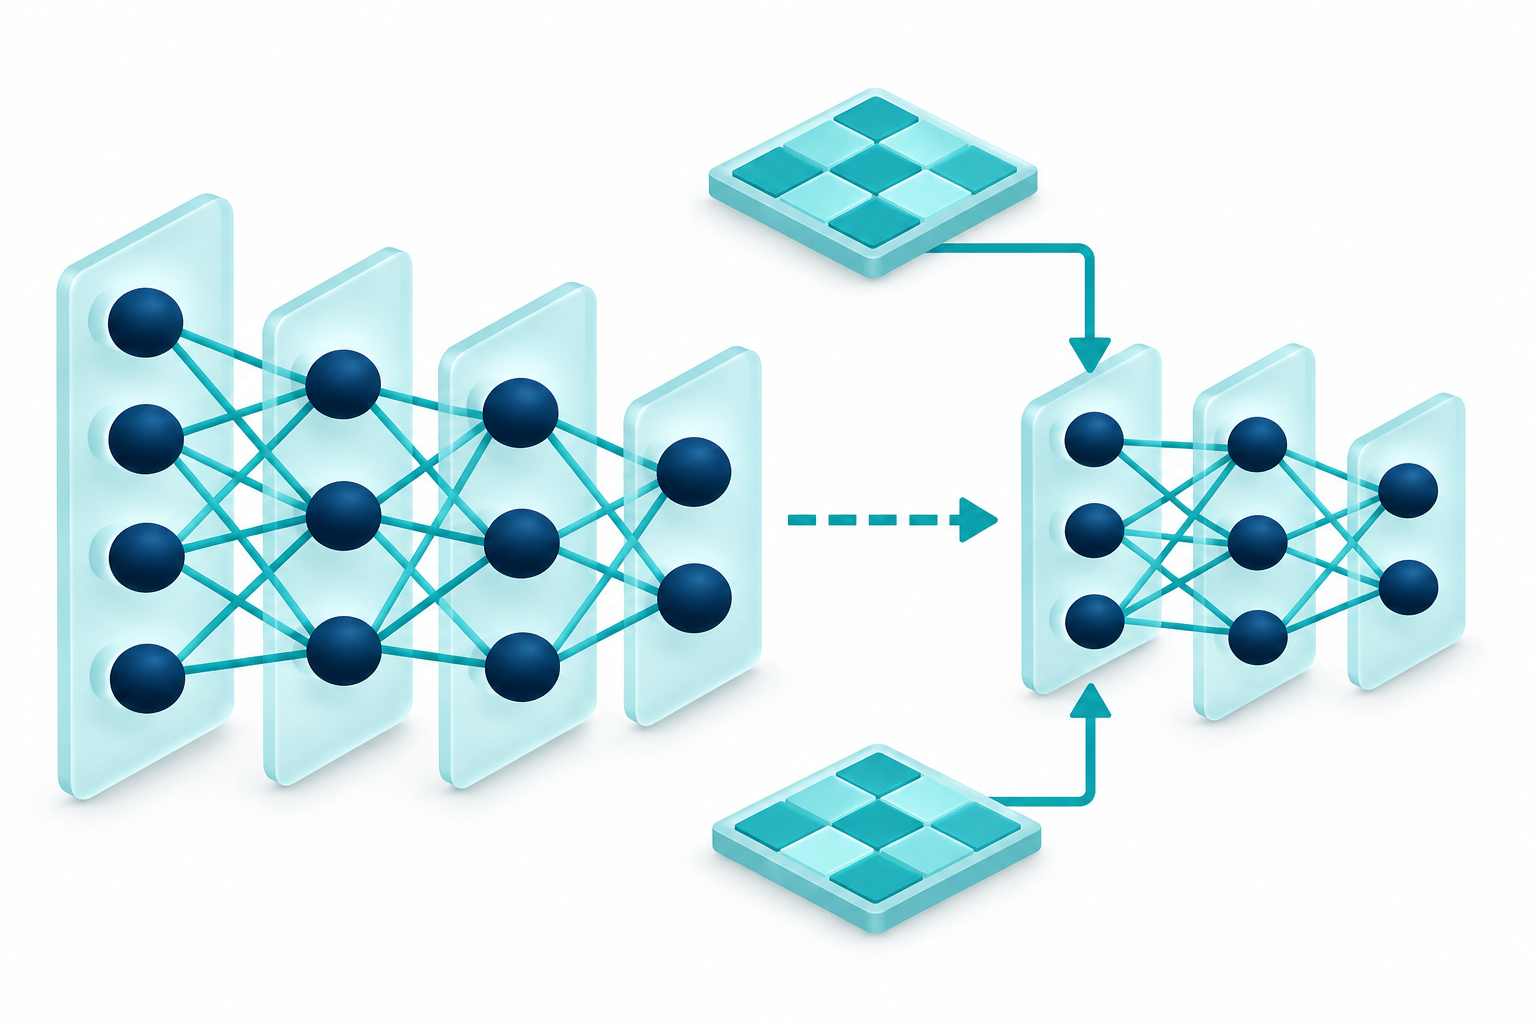
\includegraphics[width=4.0cm,height=2.45cm,keepaspectratio]{assets/illustrations/objective/understand-imagegen-v1.png}};
    \node[inner sep=0pt] at (7.4,3.32)
      {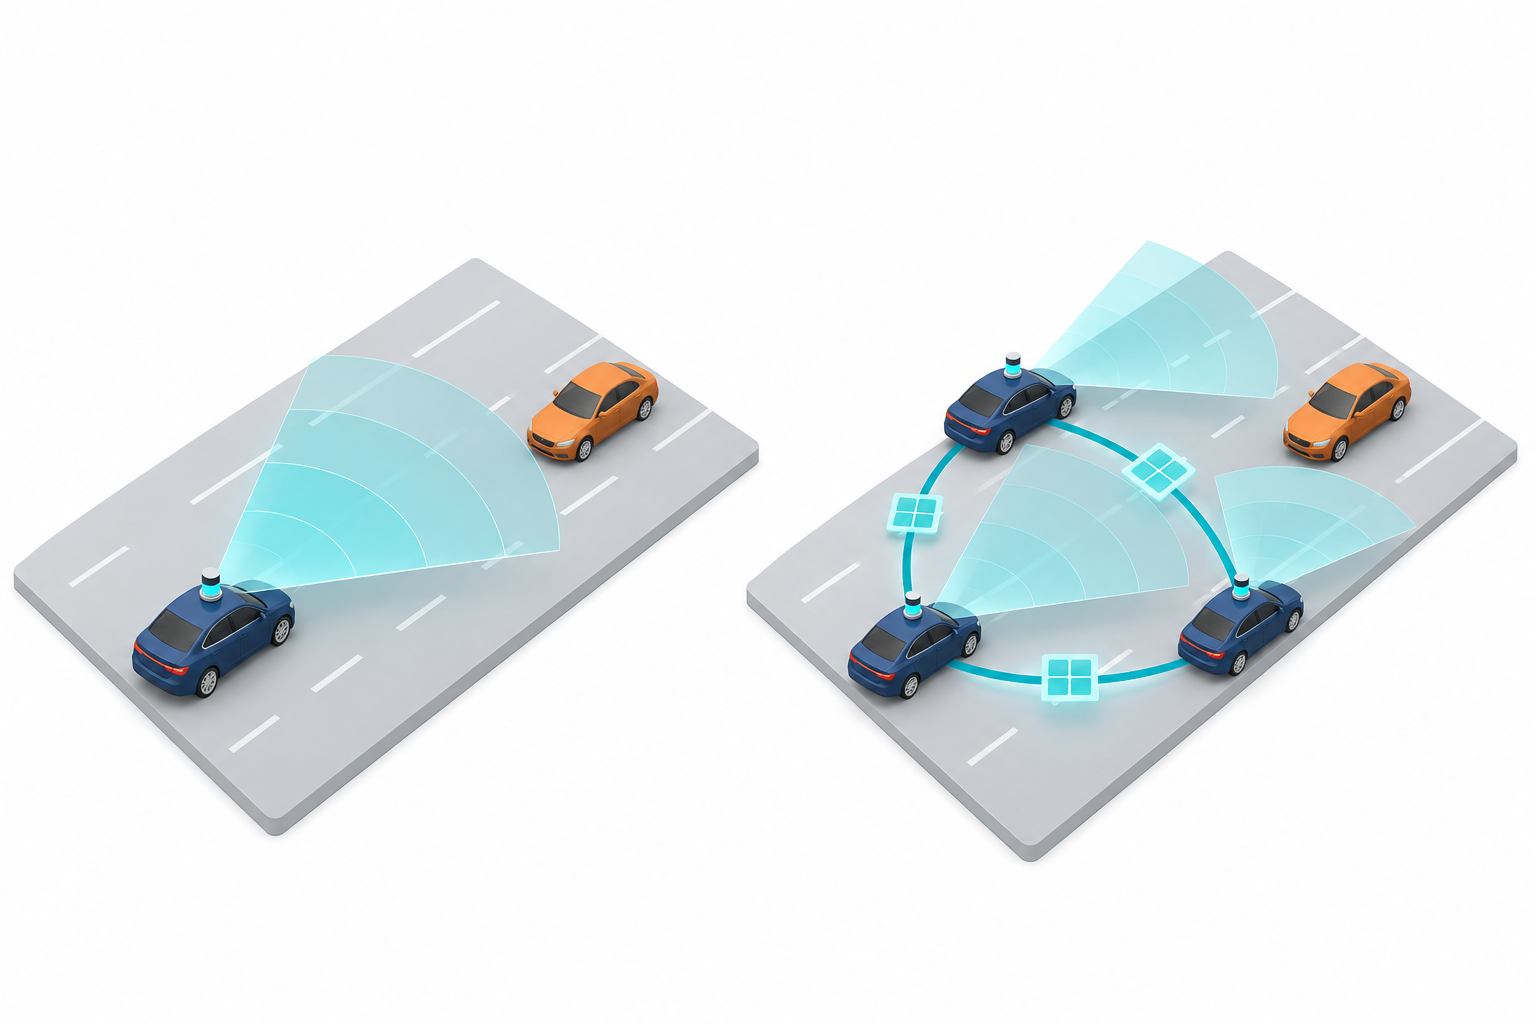
\includegraphics[width=4.0cm,height=2.45cm,keepaspectratio]{assets/illustrations/objective/compare-imagegen-v1.png}};
    \node[inner sep=0pt] at (12.4,3.32)
      {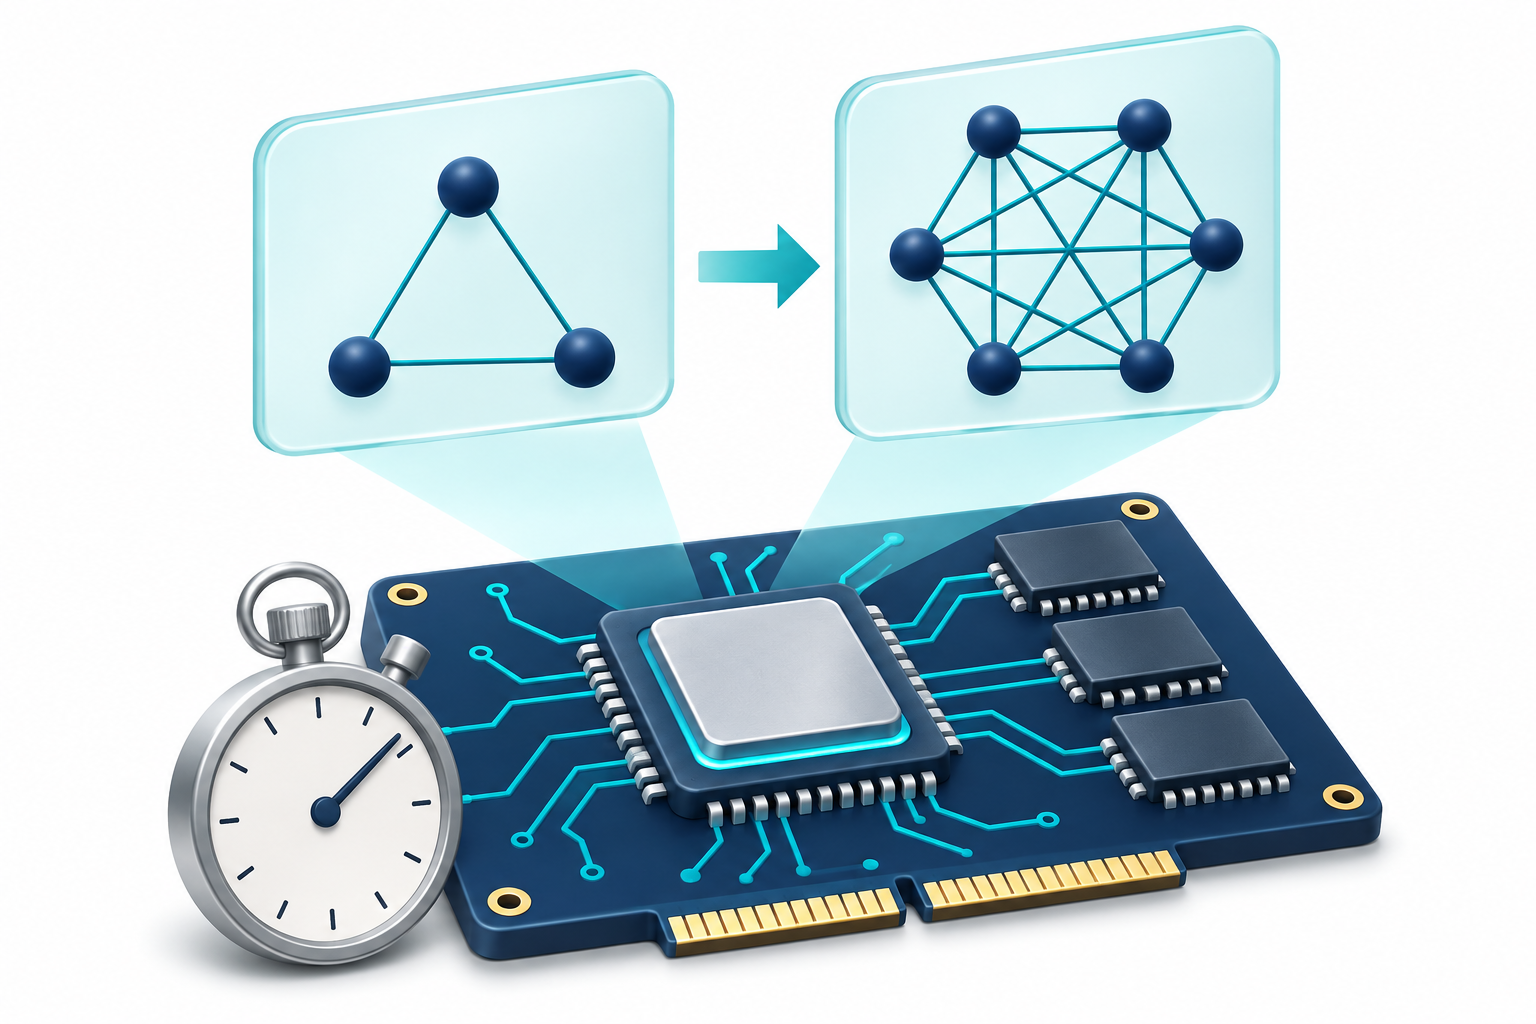
\includegraphics[width=4.0cm,height=2.45cm,keepaspectratio]{assets/illustrations/objective/benchmark-imagegen-v1.png}};
    \draw[visual arrow] (4.55,3.32) -- (5.25,3.32);
    \draw[visual arrow] (9.55,3.32) -- (10.25,3.32);
    \node[final heading] at (2.4,1.80) {Understand};
    \node[final heading] at (7.4,1.80) {Compare};
    \node[final heading] at (12.4,1.80) {Benchmark};
    \node[final caption,text width=4.4cm,
      font=\fontsize{11}{14}\selectfont] at (2.4,0.98)
      {Teacher--Student Pipeline\\and Feature Fusion};
    \node[final caption,text width=4.4cm,
      font=\fontsize{11}{14}\selectfont] at (7.4,0.98)
      {Individual vs.\\Cooperative Detection};
    \node[final caption,text width=4.4cm,
      font=\fontsize{11}{14}\selectfont] at (12.4,0.98)
      {Accuracy and Cost\\as $n$ Increases};
    \node[visual small,anchor=center] at (7.4,0.15)
      {$n$ = Number of Cooperating Agents};
  \end{VisualCanvas}}
  \SlideSource{Source: AI generated illustrations.}
\end{frame}
